\chapter{Data acquisition for CHIPS}
\label{chap:daq}


\section{Things to talk about}


\section{Diagrams}

\begin{figure}
    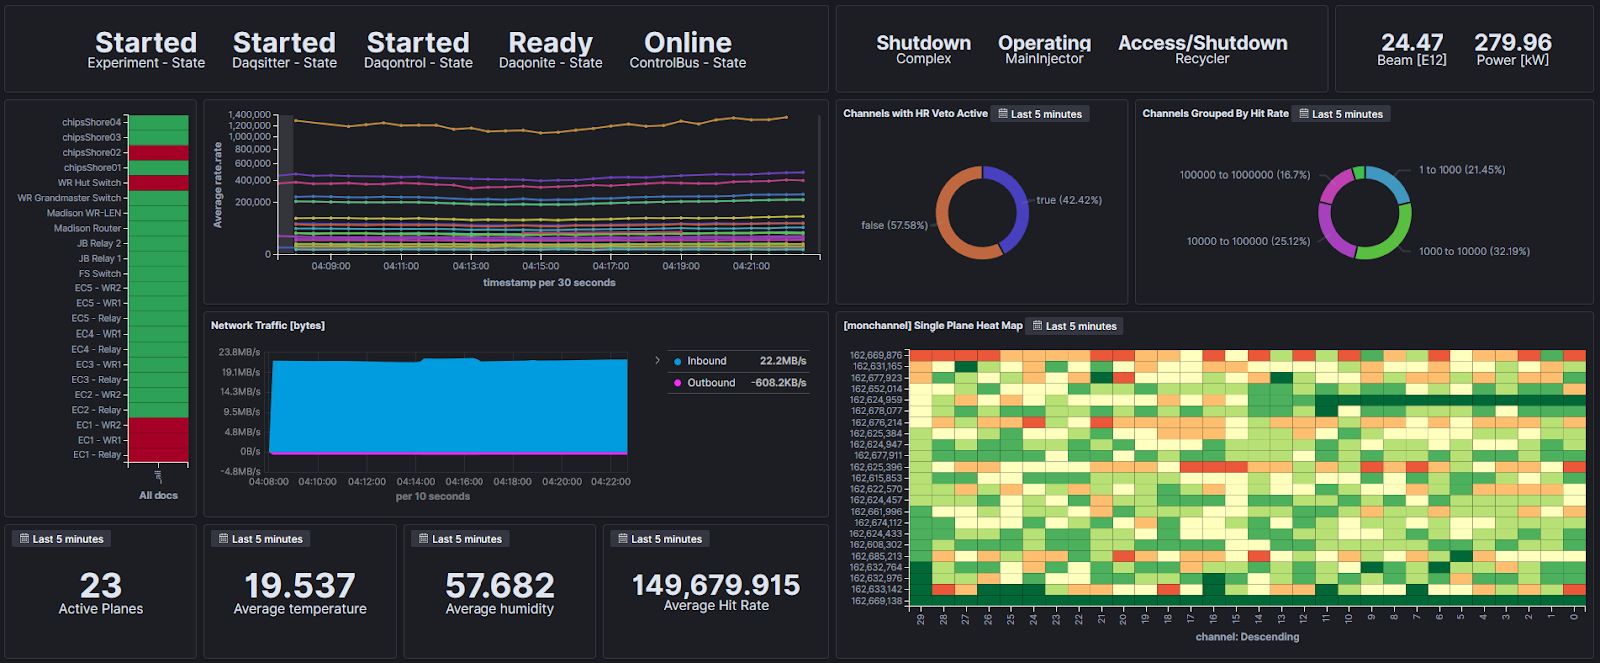
\includegraphics[width=\textwidth]{diagrams/5-daq/monitoring.png}
    \caption[monitoring short]{monitoring long}
    \label{fig:monitoring}
\end{figure}

\begin{figure}
    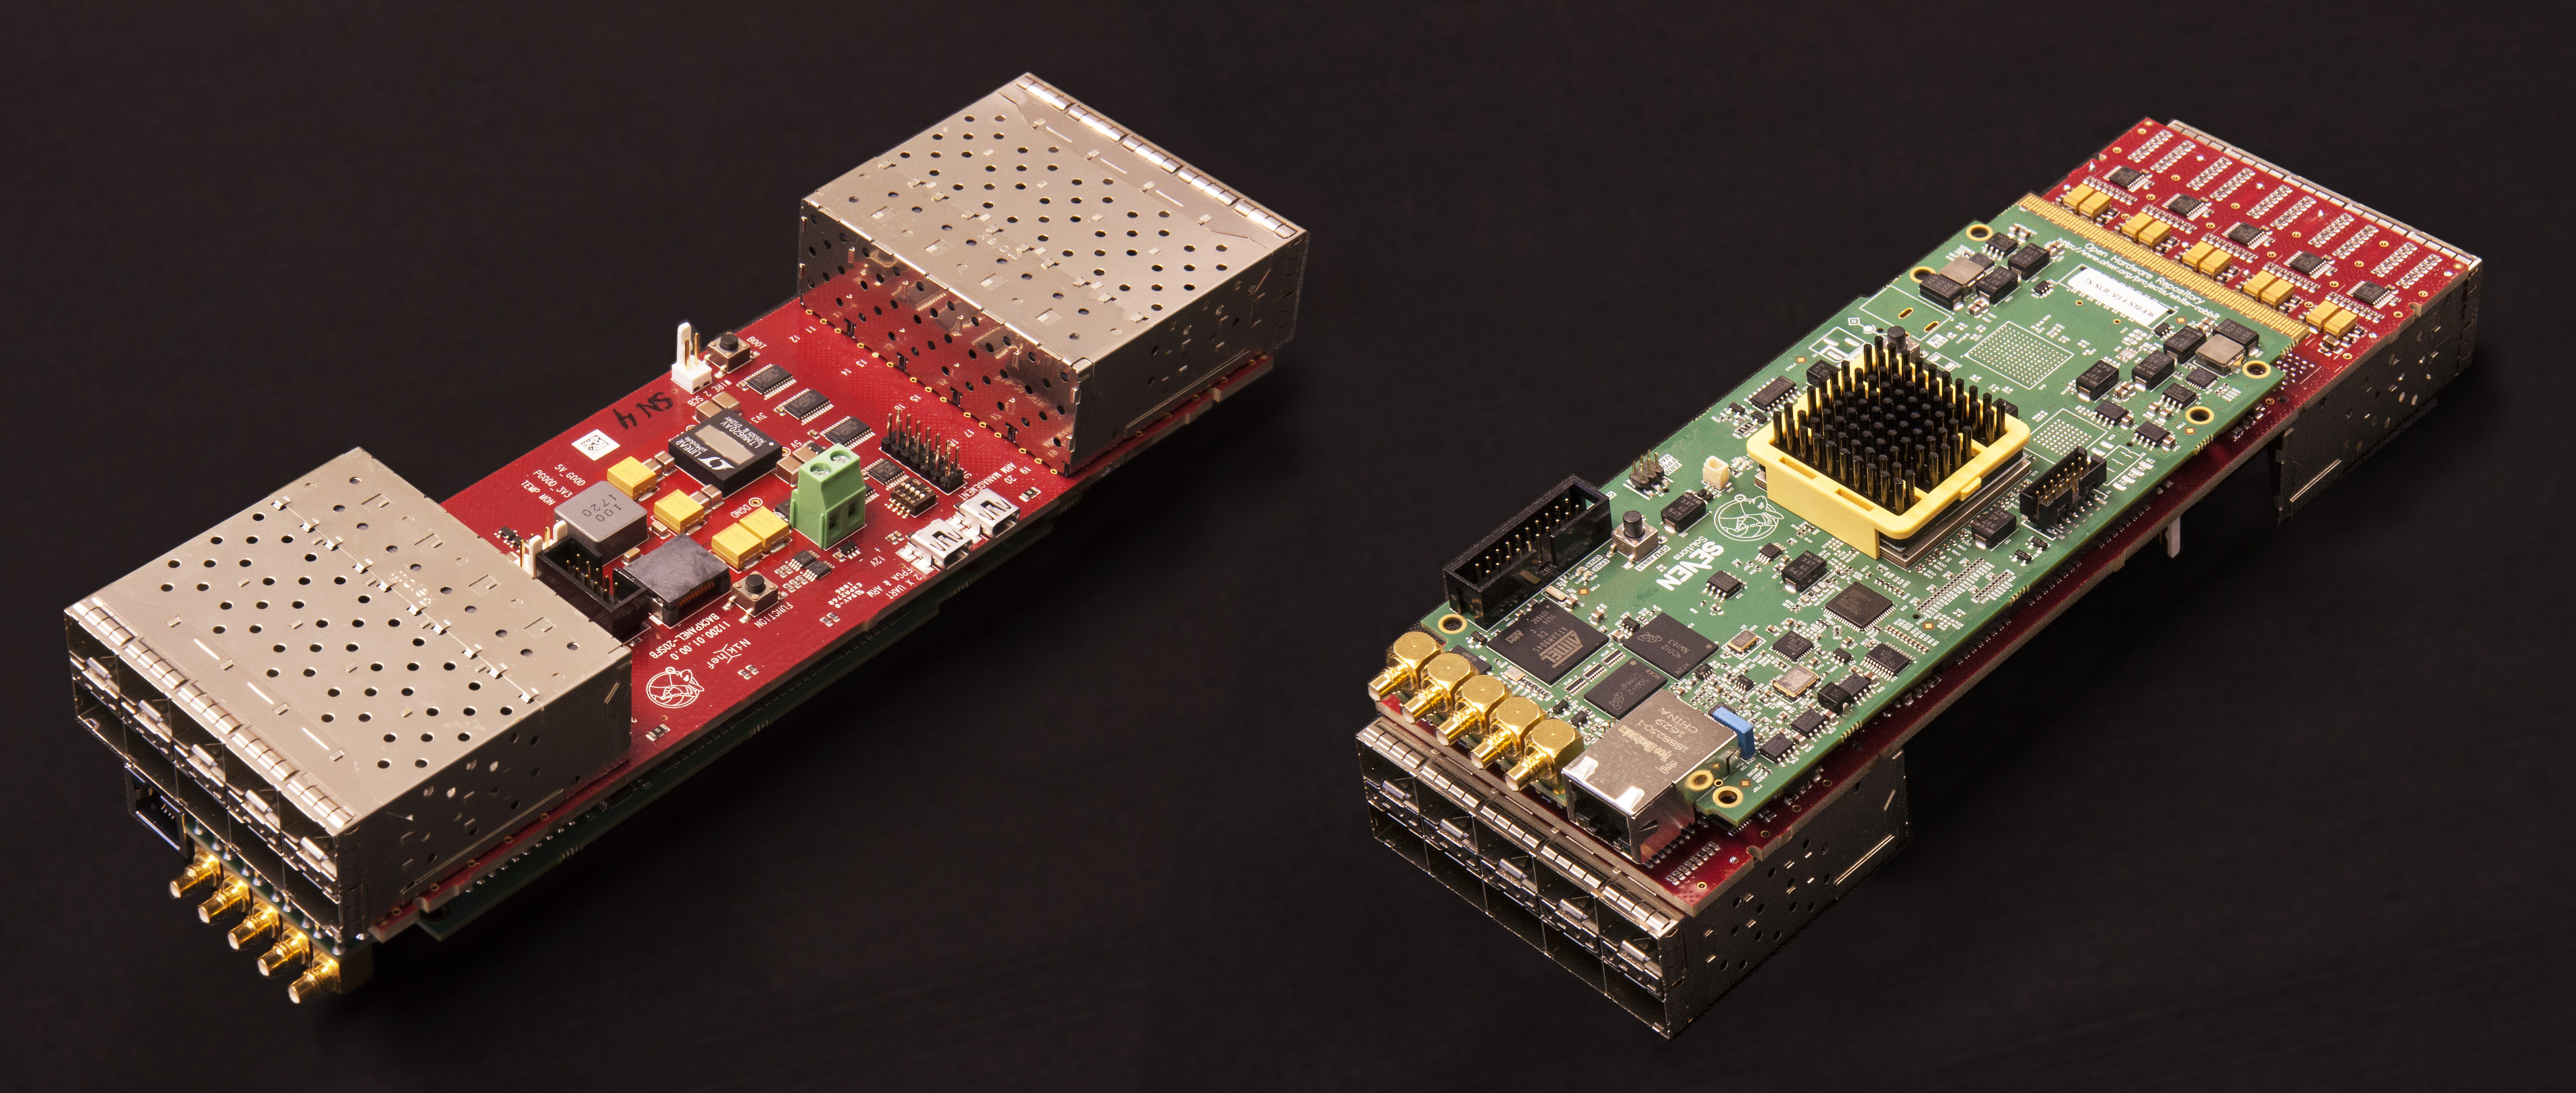
\includegraphics[width=\textwidth]{diagrams/5-daq/wr_switch.jpg}
    \caption[wr switch short]{wr switch long}
    \label{fig:wr_switch}
\end{figure}

\begin{figure}
    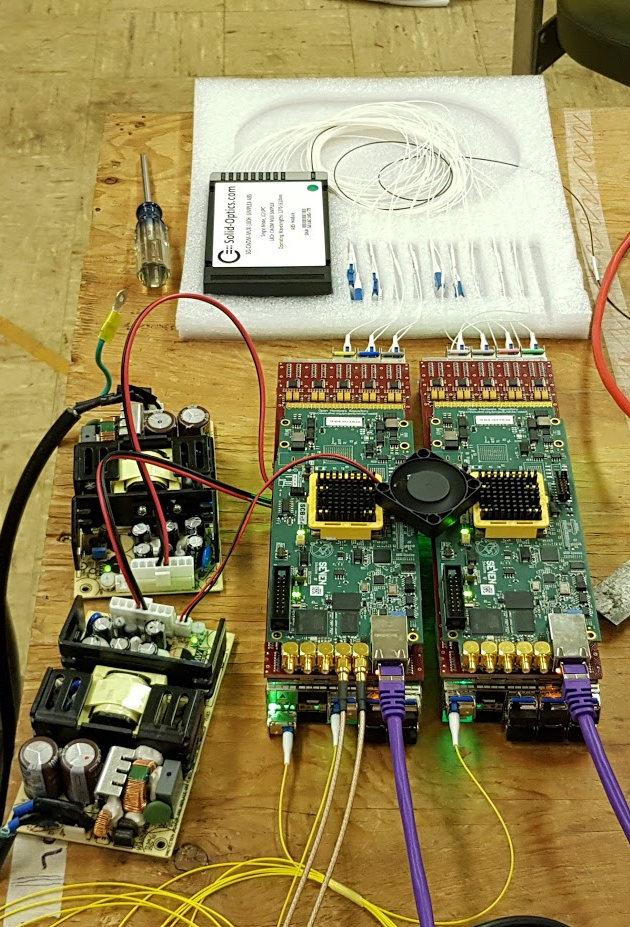
\includegraphics[width=0.8\textwidth]{diagrams/5-daq/wr_gm.jpg}
    \caption[wr gm short]{wr gm long}
    \label{fig:wr_gm}
\end{figure}

\begin{figure}
    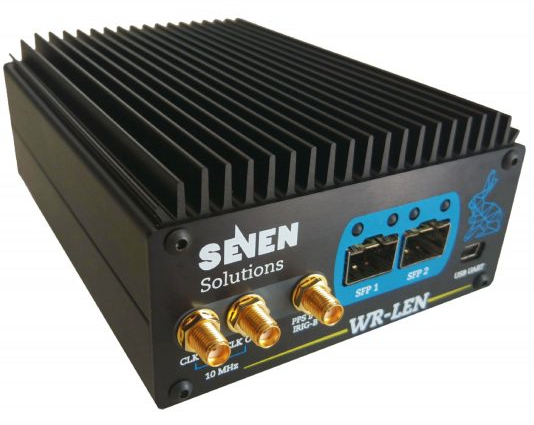
\includegraphics[width=0.8\textwidth]{diagrams/5-daq/wr_len.jpg}
    \caption[wr len short]{wr len long}
    \label{fig:wr_len}
\end{figure}

\begin{figure}
    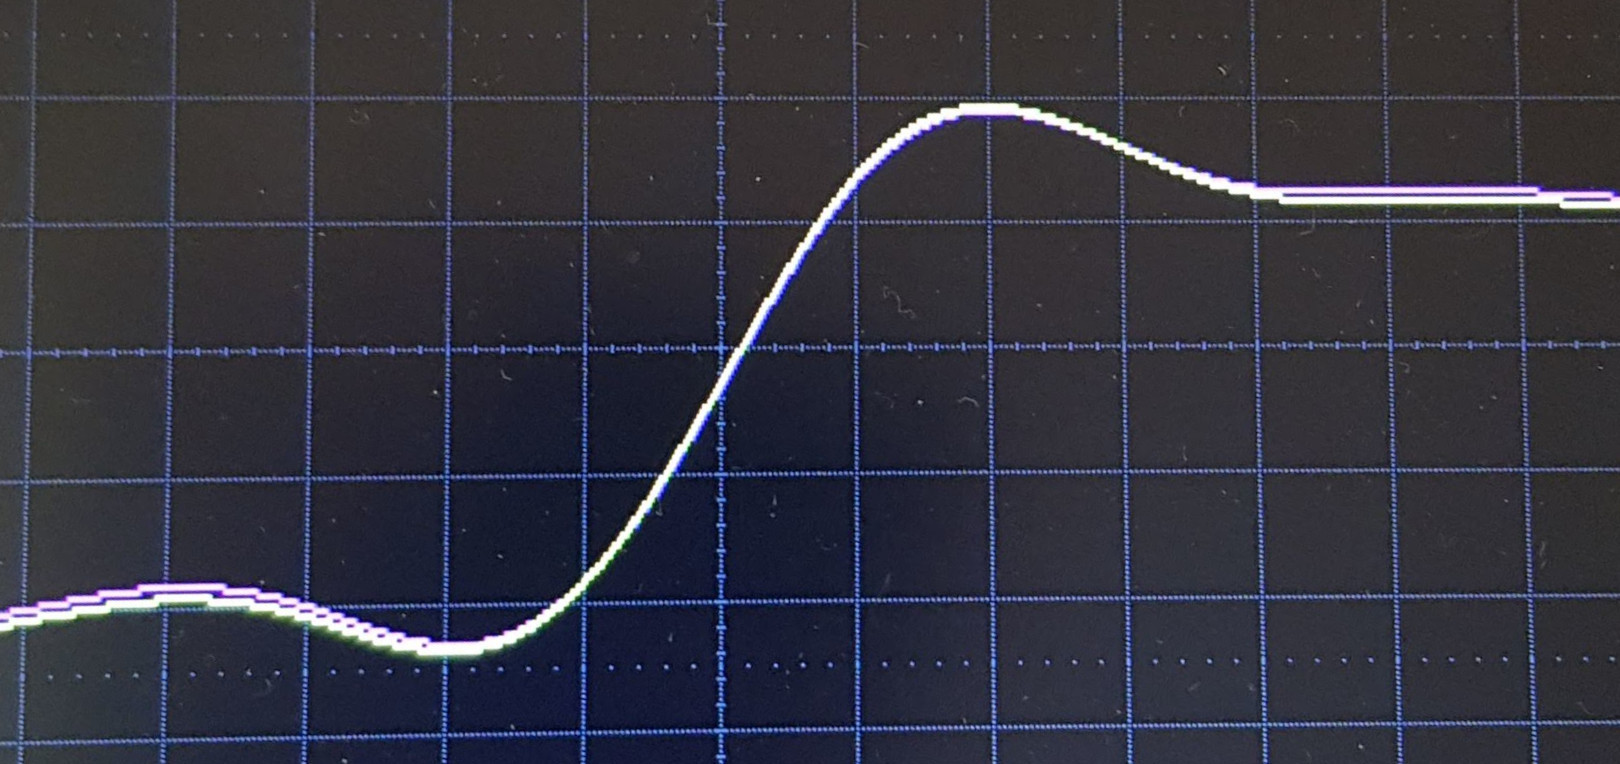
\includegraphics[width=0.8\textwidth]{diagrams/5-daq/sync.jpg}
    \caption[sync short]{sync long}
    \label{fig:sync}
\end{figure}

\begin{figure}[htp]
    \centering
    \subcaptionbox{nikhef pmt\label{fig:nikhef_pmt}}{%
        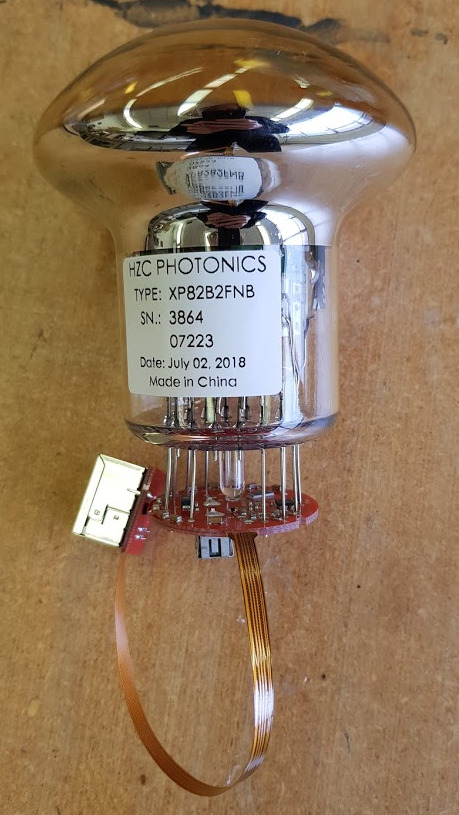
\includegraphics[height=10cm]{diagrams/5-daq/nikhef_pmt.jpg}%
    }
    \quad
    \subcaptionbox{clb\label{fig:clb}}{%
        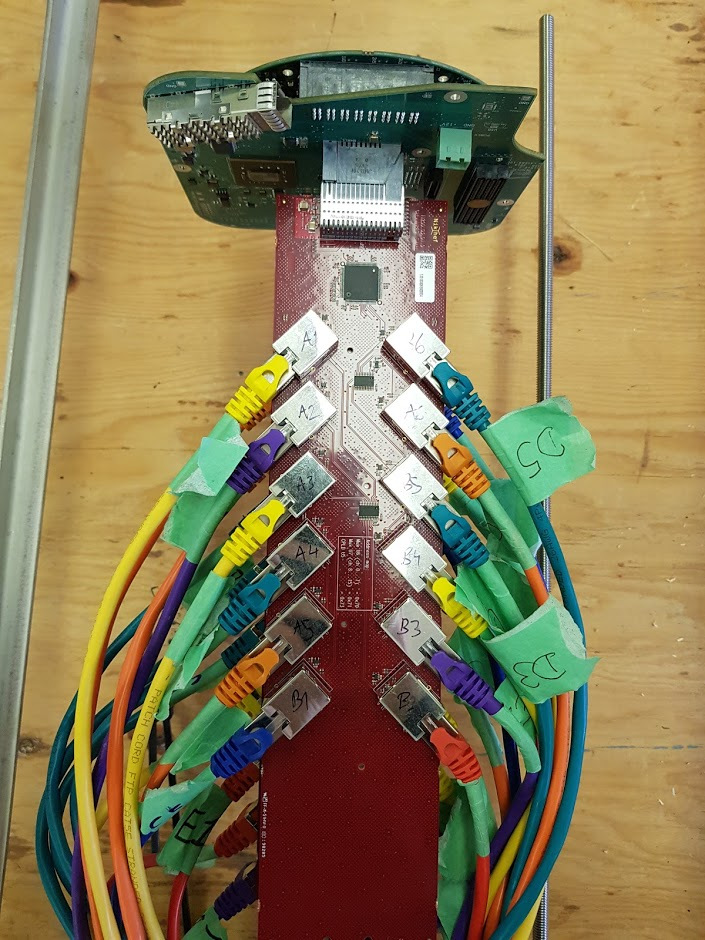
\includegraphics[height=10cm]{diagrams/5-daq/clb.jpg}%
    }
    \caption{The caption}
\end{figure}

\begin{figure}[htp]
    \centering
    \subcaptionbox{pmt disassembled\label{fig:pmt_disassembled}}{%
        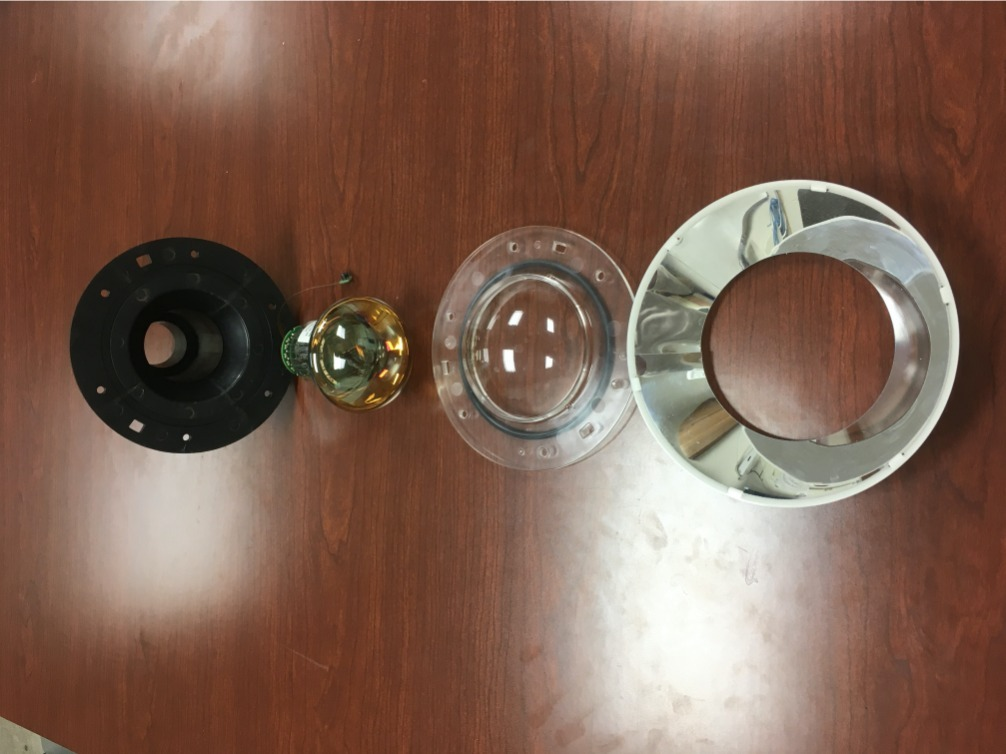
\includegraphics[height=5cm]{diagrams/5-daq/pmt_disassembled.jpg}%
    }
    \quad
    \subcaptionbox{pmt assembled\label{fig:pmt_assembled}}{%
        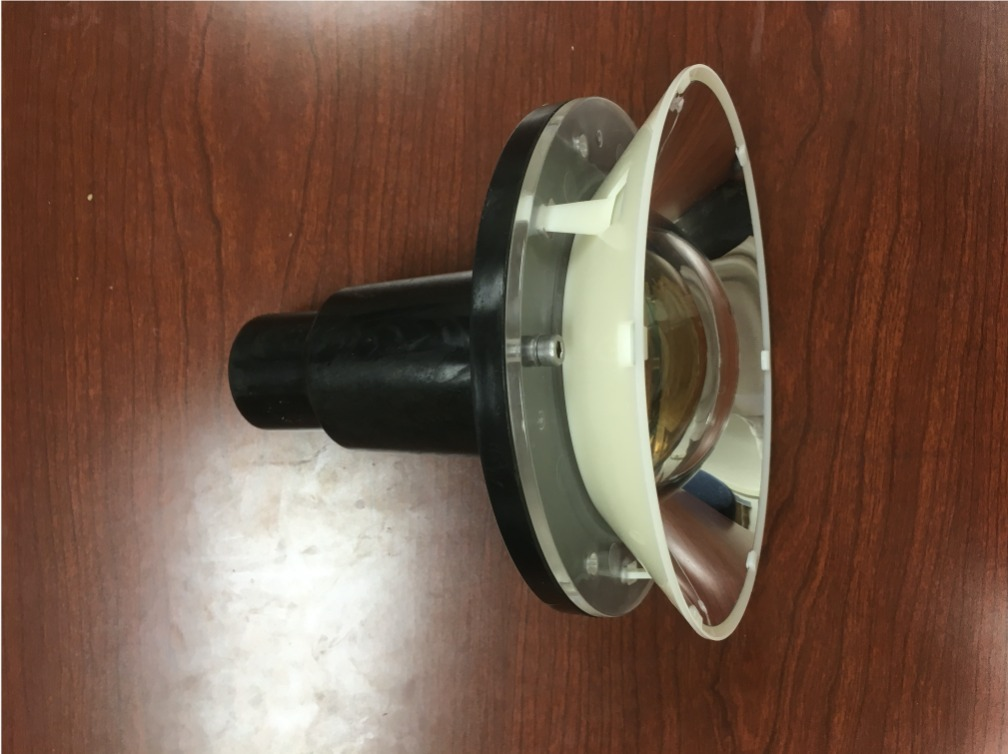
\includegraphics[height=5cm]{diagrams/5-daq/pmt_assembled.jpg}%
    }
    \caption{The caption}
\end{figure}

\begin{figure}
    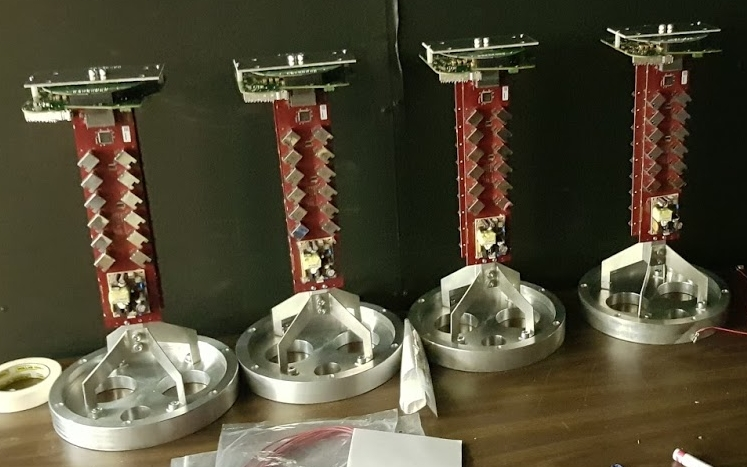
\includegraphics[width=0.8\textwidth]{diagrams/5-daq/rockets.jpg}
    \caption[rockets short]{rockets long}
    \label{fig:rockets}
\end{figure}

\begin{figure}
    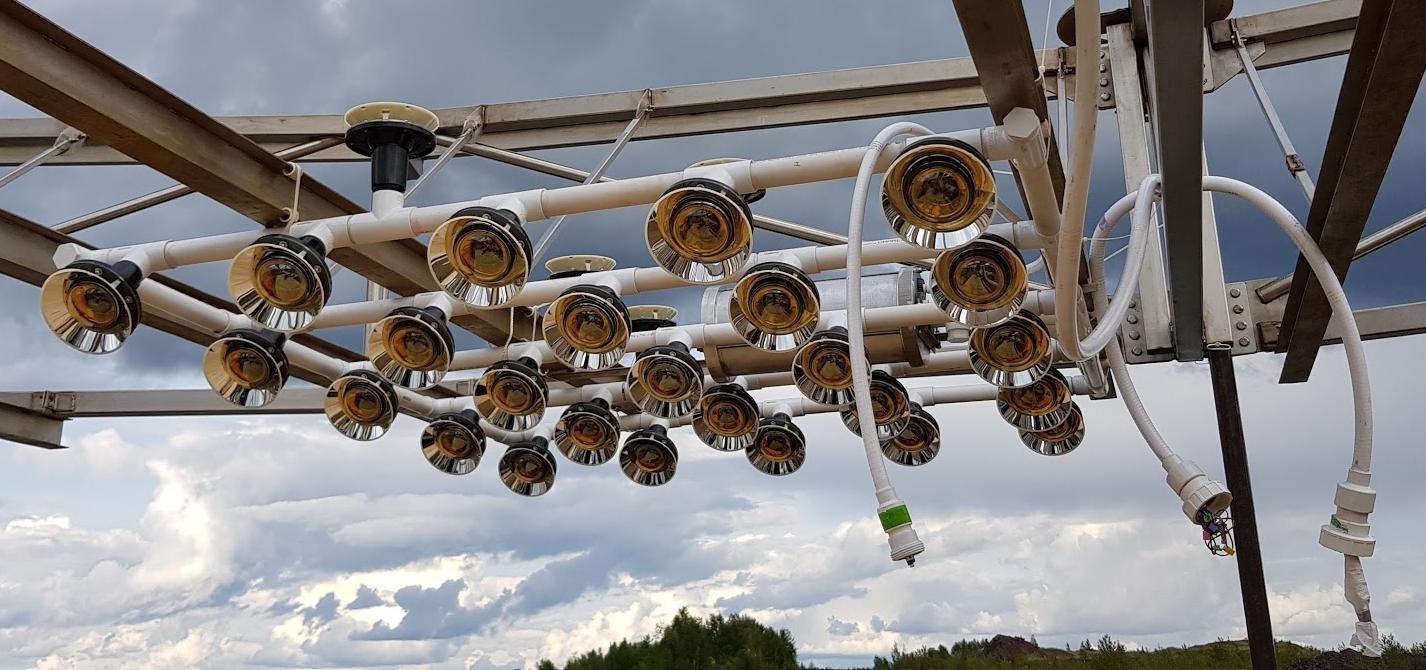
\includegraphics[width=0.8\textwidth]{diagrams/5-daq/single_plane.jpg}
    \caption[single plane short]{single plane long}
    \label{fig:single_plane}
\end{figure}

\begin{figure}
    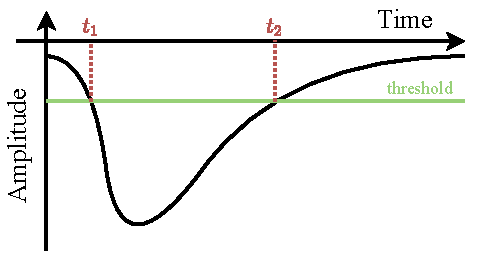
\includegraphics[width=0.8\textwidth]{diagrams/5-daq/tot.pdf}
    \caption[tot short]{tot long}
    \label{fig:tot}
\end{figure}

\begin{figure}[htp]
    \centering
    \subcaptionbox{beaglebone\label{fig:beaglebone}}{%
        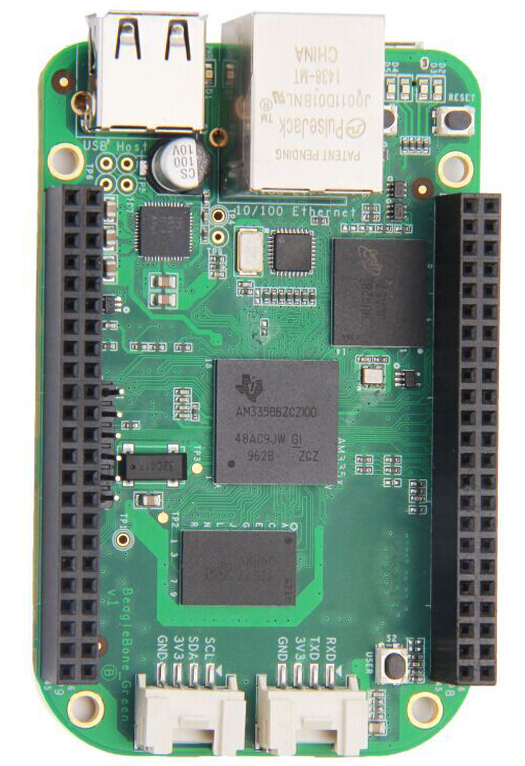
\includegraphics[height=7cm]{diagrams/5-daq/beaglebone.jpg}%
    }
    \quad
    \subcaptionbox{danout\label{fig:danout}}{%
        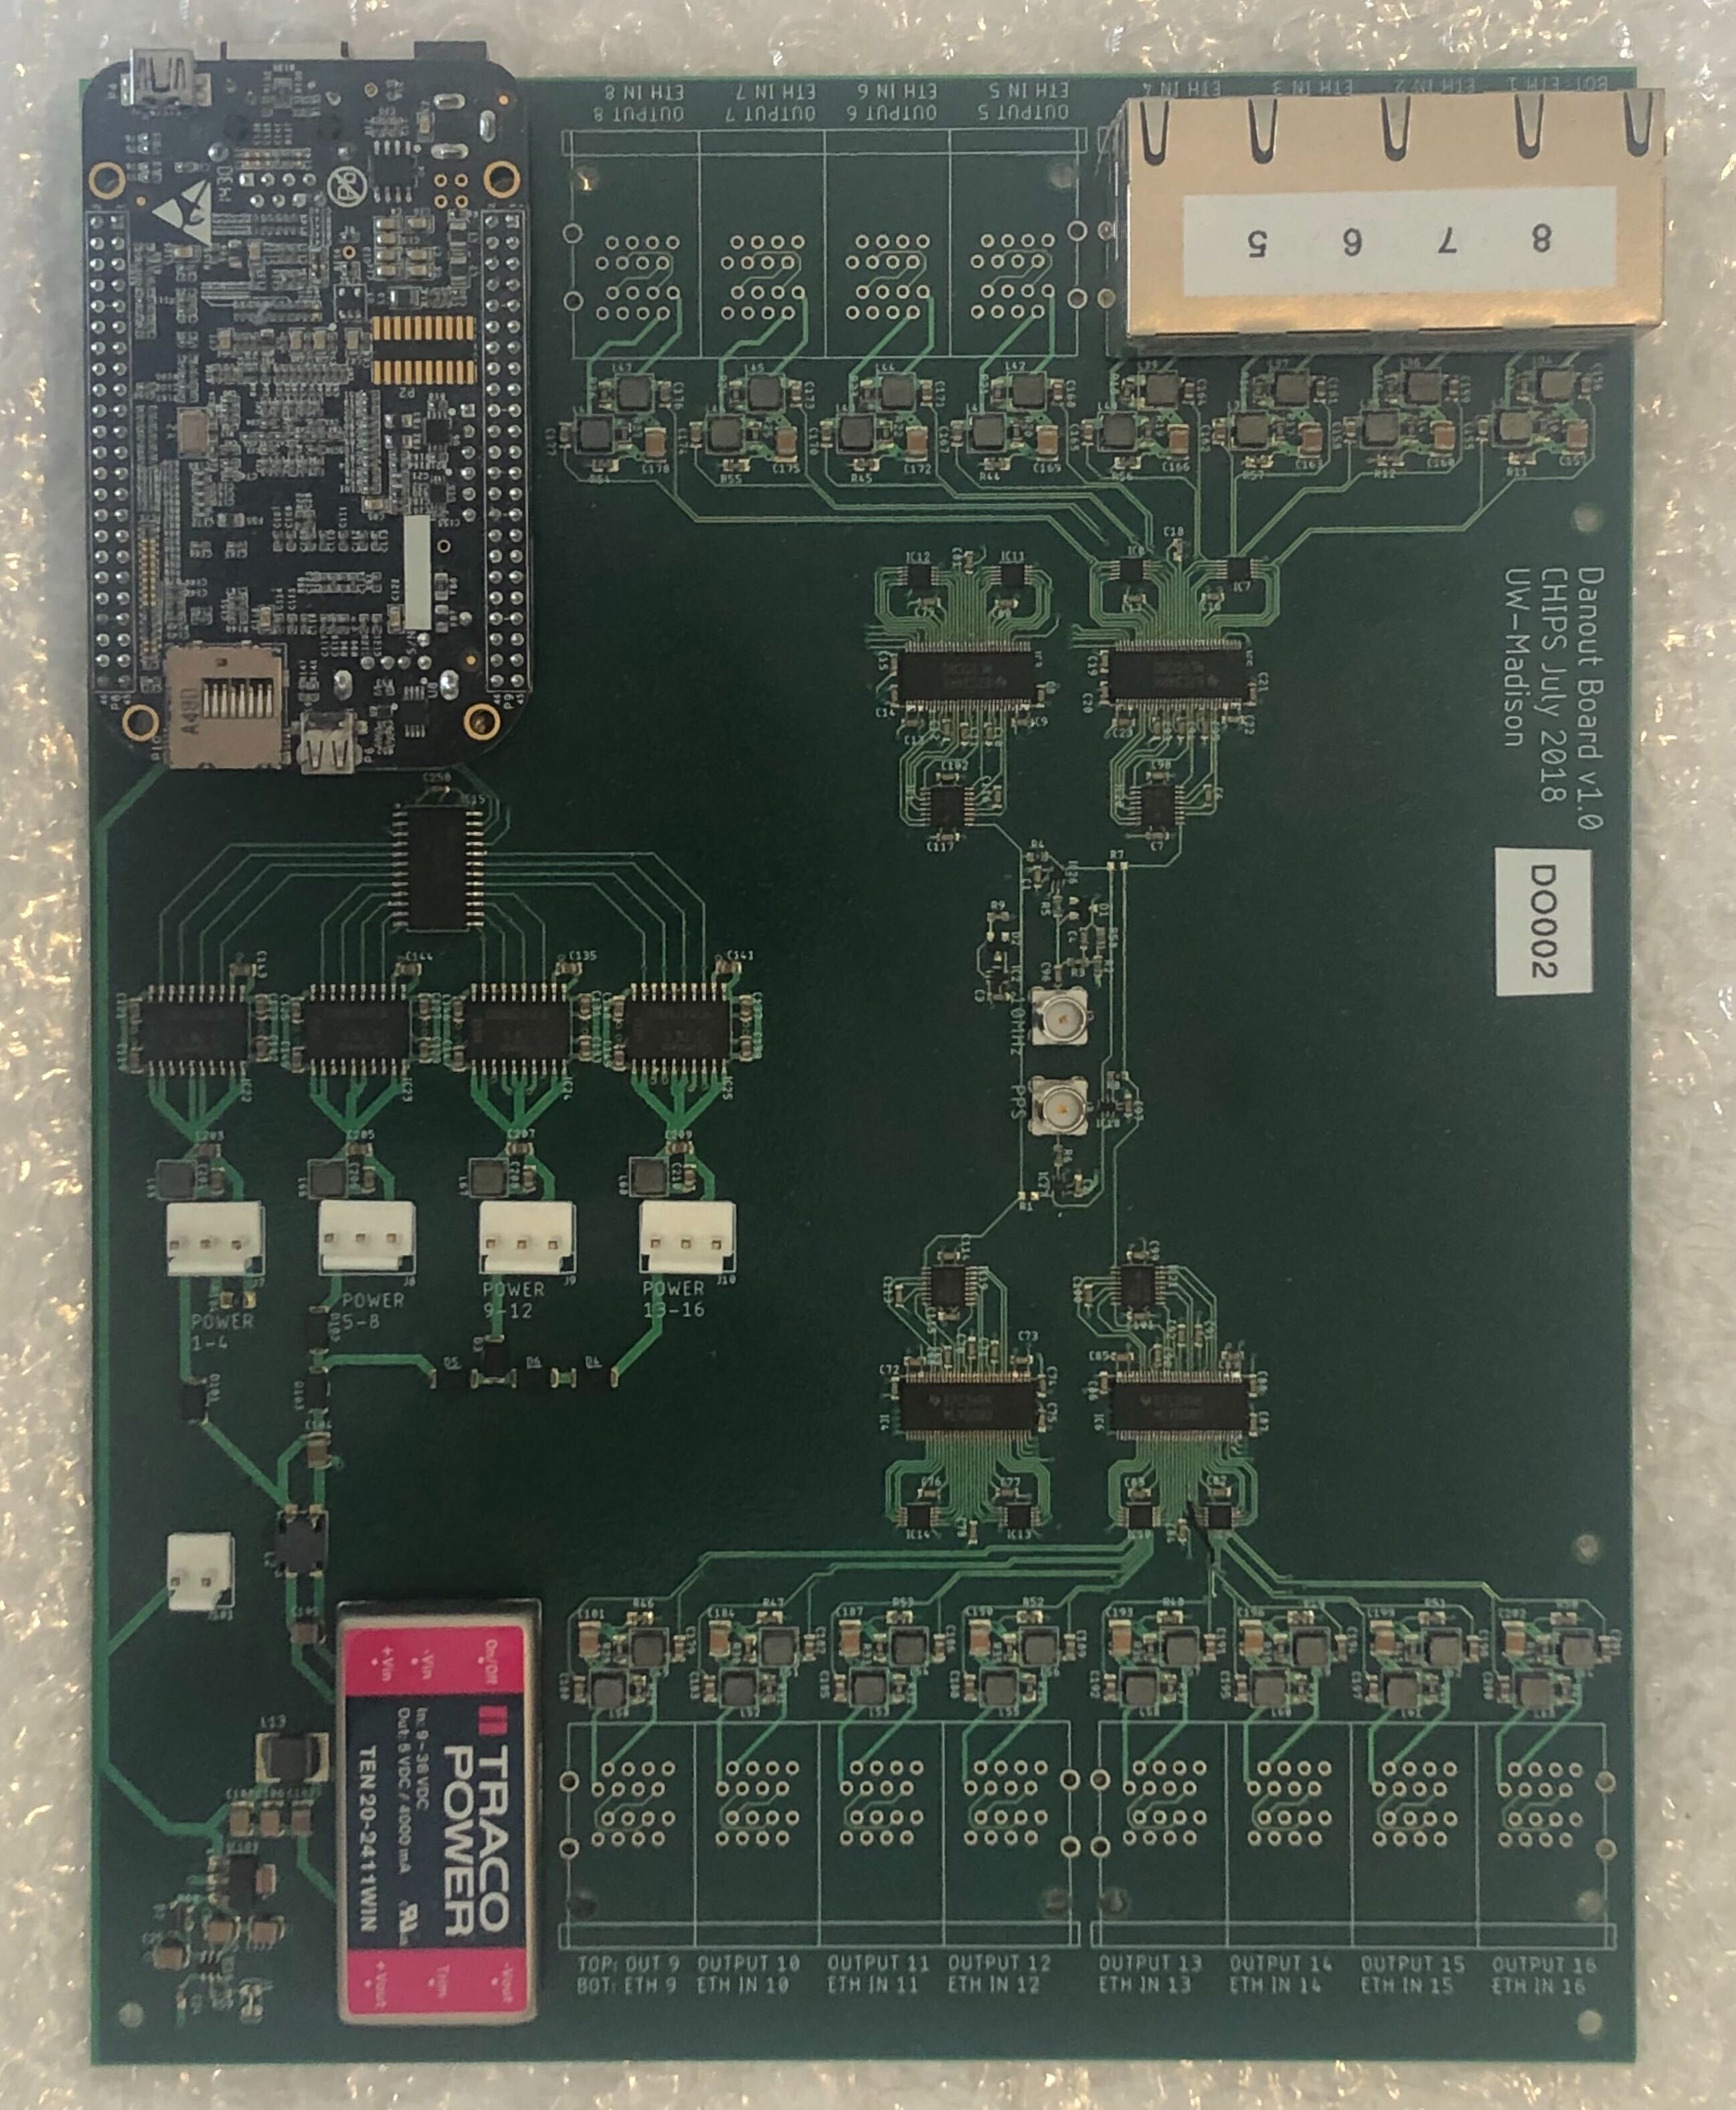
\includegraphics[angle=90, height=7cm]{diagrams/5-daq/danout.jpg}%
    }
    \caption{The caption}
\end{figure}

\begin{figure}
    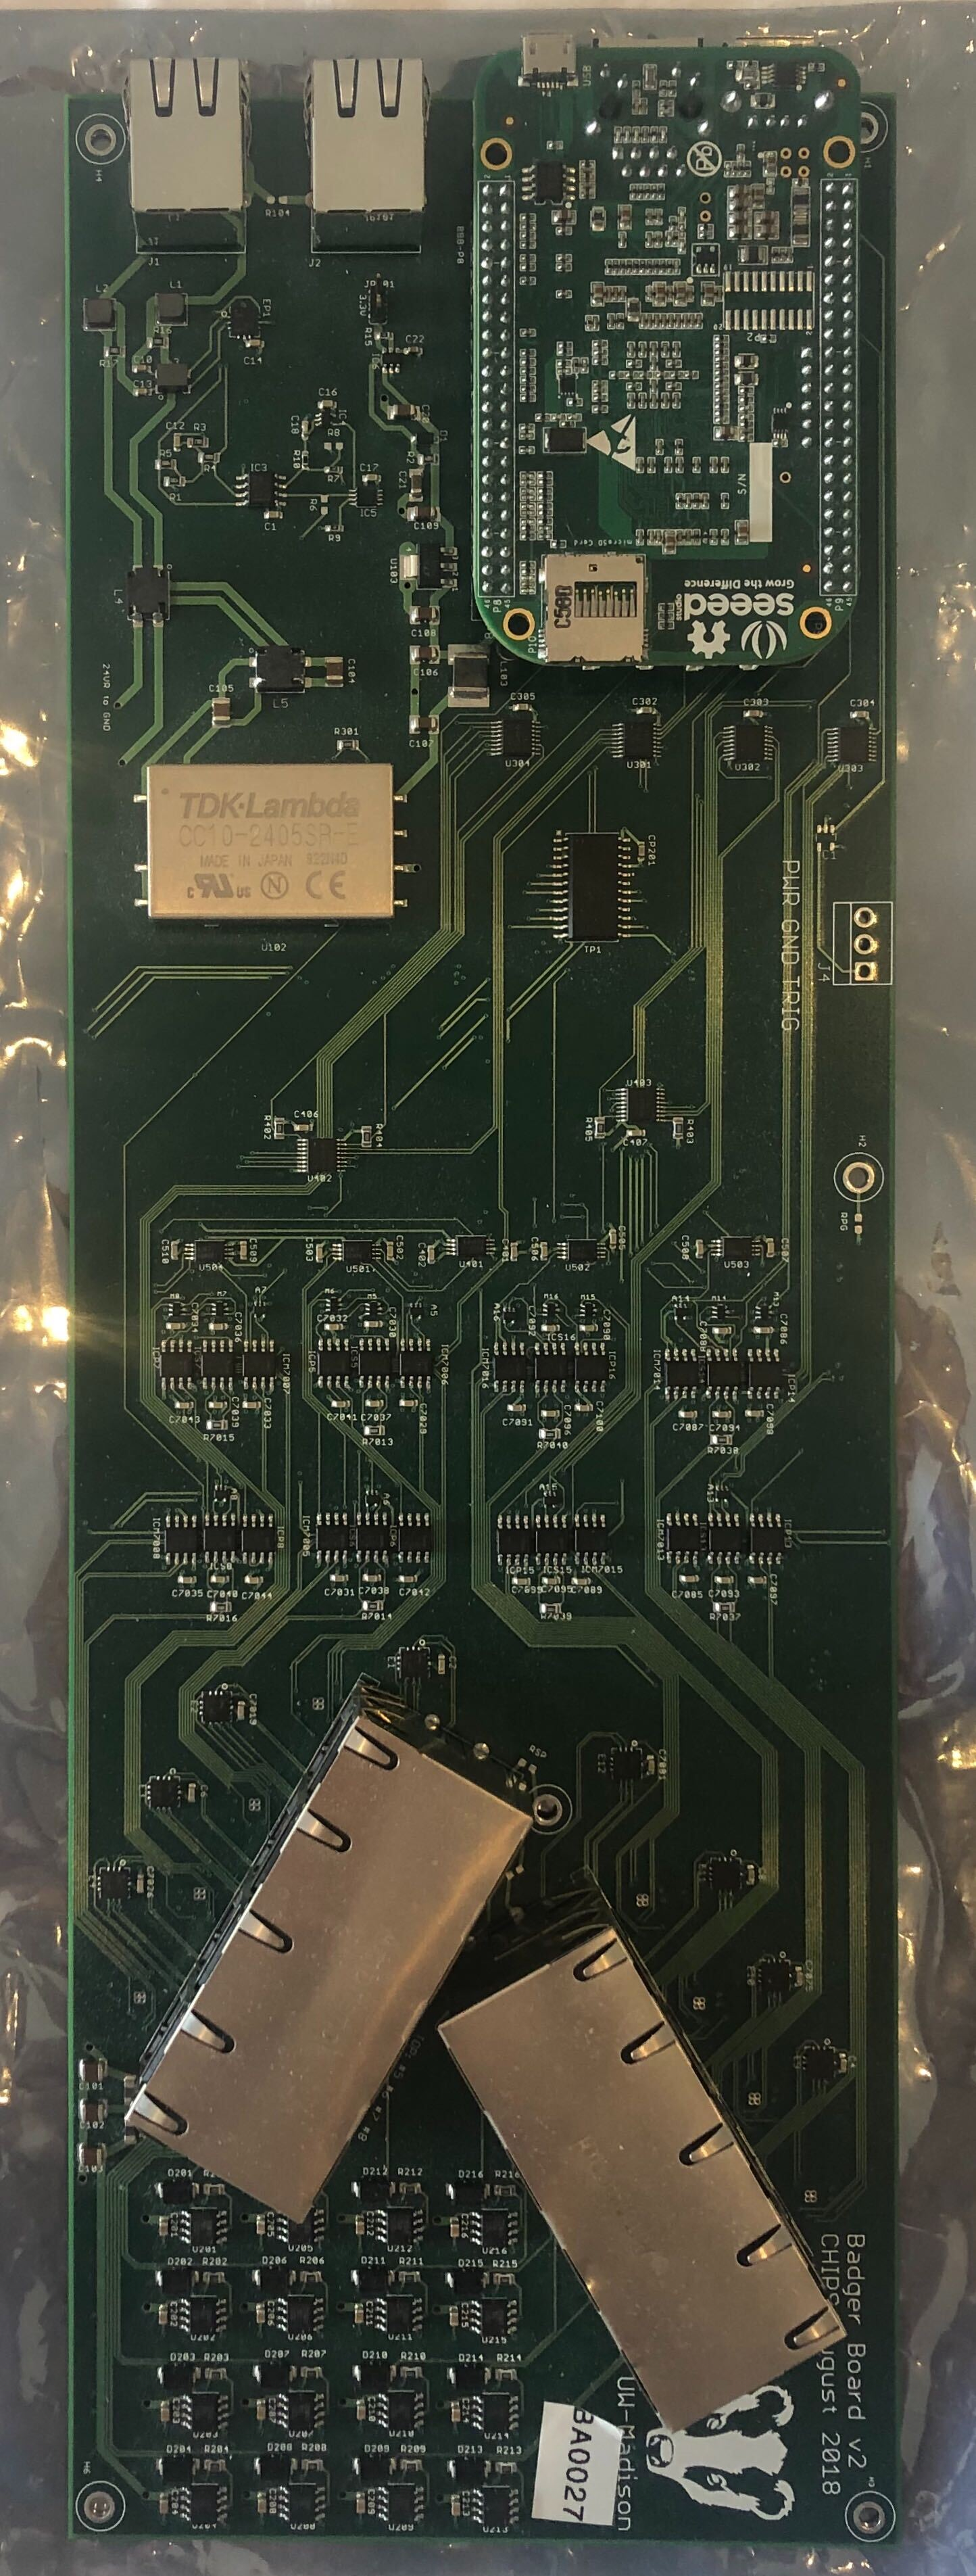
\includegraphics[angle=90,origin=c,width=\textwidth]{diagrams/5-daq/badger.jpg}
    \caption[badger short]{badger long}
    \label{fig:badger}
\end{figure}

- Madison Diagrams
- Nikhef Diagrams
- Hut Diagrams
- Jelly box Diagrams
- Electronics box Diagrams
- Manifold diagram, with electronics box layout
- DAQ software diagram
- Finite state machine diagram
- Monitoring diagram elastic stack
- Spill server diagram, probably combined with another diagram

\section{References}

- WR Papers
- km3net daq Papers
- PMT time resolution Papers

\section{Reference notes}